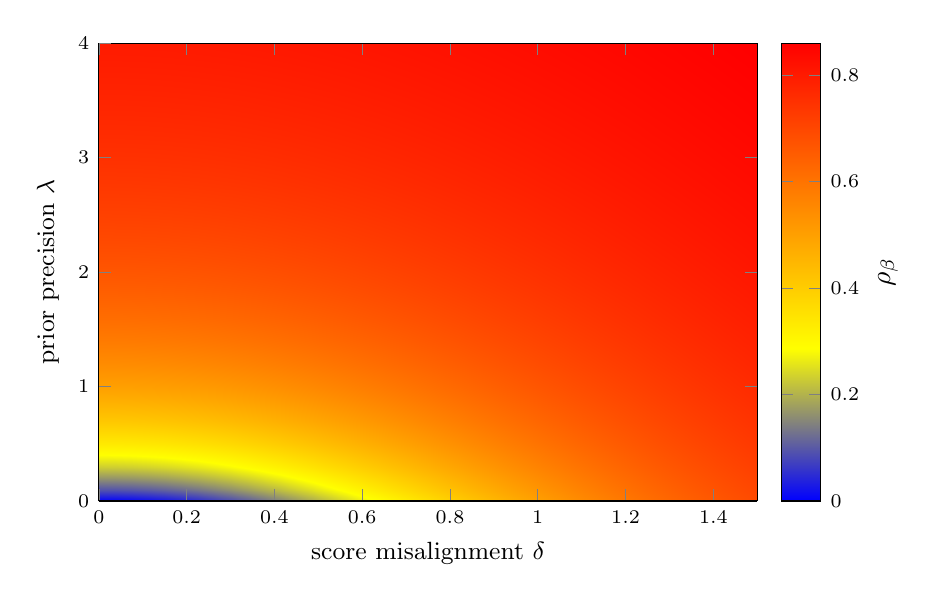
\begin{tikzpicture}
\begin{axis}[
 width=0.82\columnwidth,height=0.61\columnwidth,
 view={0}{90},xmin=0,xmax=1.5,ymin=0,ymax=4,
 xlabel={score misalignment $\delta$},ylabel={prior precision $\lambda$},
 colorbar,colorbar style={ylabel={$\rho_\beta$},yticklabel style={font=\scriptsize}},
 point meta min=0,point meta max=0.86,
 tick label style={font=\scriptsize},label style={font=\small}]
\addplot3[surf,shader=interp,domain=0:1.5,domain y=0:4,samples=41]
 {(x^2+y)/(1+x^2+y)};
\end{axis}
\end{tikzpicture}
